
\begin{frame} 
  \titlepage 
\end{frame} 

\begin{frame}{Disclaimer}
  \Large{Неофициальное содержание:}
  \begin{itemize}
    \item \normalsize{расисткие сплетни о коммерческих вендорах}
    \item анальное огораживание частных недо-серверов 
    \item убедительное обоснование пионерских поделок
    \item неприкрытая реклама side-проекта MLUG
  \end{itemize}


  \emph{ }\newline \pause

  Автор доклада гарантирует эмоционально окрашенные субьективные оценки.
\end{frame}

\begin{frame}{Краткое содержание, официально}
  \tableofcontents
  % You might wish to add the option [pausesections]
\end{frame}

\section{Технология XMPP/Jabber}

\begin{frame}{Общие сведения}
  \Large{«Православие,\\Самодержавие,\\Народность»} 
\end{frame}

\begin{frame}{Общие сведения}
  \Large{ \sout{«Православие,\\Самодержавие,\\Народность»} }

  «Открытые протоколы,\\ Децентрализация,\\Instant Messaging and Presence»

\end{frame}

\begin{frame}{Основа - протокол}
  \begin{itemize}
    \item Протокол XMPP\footnote{Extensible Messaging and Presence Protocol}

    \item Внутри XML

    \item Стандартизирован IETF\footnote{RFC 6120, RFC 6121, и RFC 6122}.

    \item Доп расширения к RFC: XEP \footnote{ ``XMPP Standarts Foundation``}
  \end{itemize}

\end{frame}

\begin{frame}{Что умеет XMPP}
  С т.ч. рядового пользователя:
  \begin{itemize}
    \item обычные и групповые чаты
    \item передача голоса и видео
    \item передача файлов
    \item серверная история
    \item одновременное подключение нескольких клиентов
  \end{itemize}
\end{frame}

\begin{frame}{Как выглядит (Psi)}
  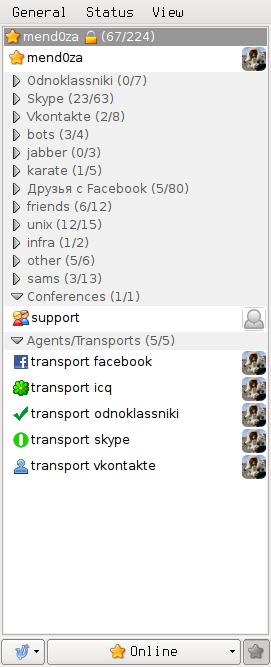
\includegraphics[height=5.9cm]{psi-plus}\emph{ }
  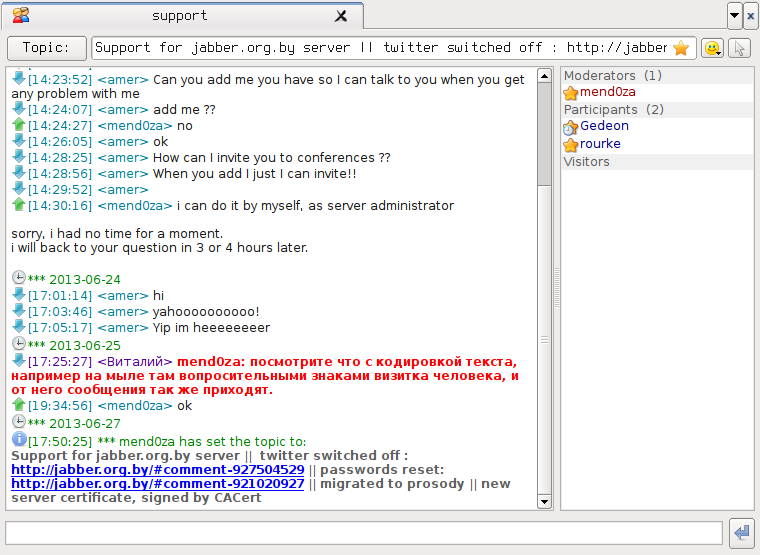
\includegraphics[height=5.9cm]{muc}
  % 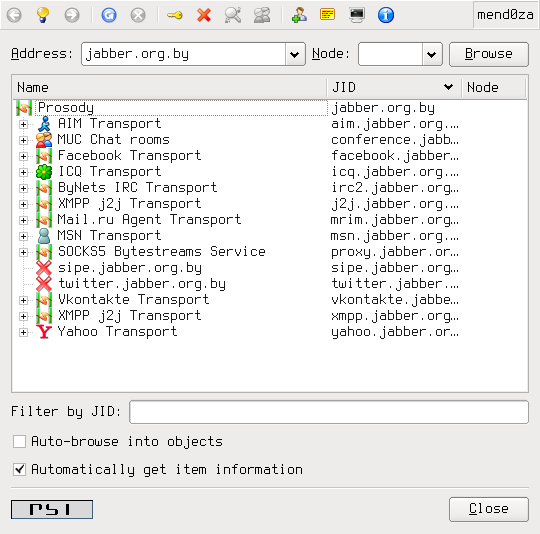
\includegraphics[height=4cm]{discovery}
\end{frame}

\begin{frame}{Базовые понятия и функции}

  \begin{block}{JID : login@server}
    Каждый сервер - независимая сущность. 

    Сервера договариваются между собой по XMPP.

    XMPP Federation или XMPP s2s.
  \end{block} \pause

  \begin{block}{Публикация статуса и подписка на него}
    Примеры: 
    \begin{enumerate}
      \item статус контакта (в сети | away | n/a)
      \item какую музыку слушает
      \item подписка на ботов (погода, новости, etc)
    \end{enumerate}
  \end{block}

\end{frame}


\begin{frame}{Наиболее интересные возможности}
  \begin{itemize}
    \item серверные шлюзы (транспорты) в другие IM\footnote{ICQ, Skype, MSN, SIP, IRC, Email, в том числе и другие XMPP}
    \item шифрование: клиент-сервер и сервер-сервер\footnote{плюс можно шифровать открывать открытым ключом}
    \item удалённая передача команд
    \item инструменты совместной работы\footnote{Abiword, Inkskape, LibreOffice, Coccinella}
    \item микроблоггинг
    \item сетевые распределённые игры
    \item geolocation
    \item cервисы авторизации: OpenID, OAuth
    \item облачные вычисления
  \end{itemize}

\end{frame}

